\documentclass[FIPLY_base.tex]{subfiles}

\author{Gerald Irsiegler}
\date{26. Februar 2016}

\begin{document}
\section{Übungskatalog}

\subsection{Beschreibung}
Der Übungskatalog beinhaltet eine Liste aller verfügbaren Übungen.

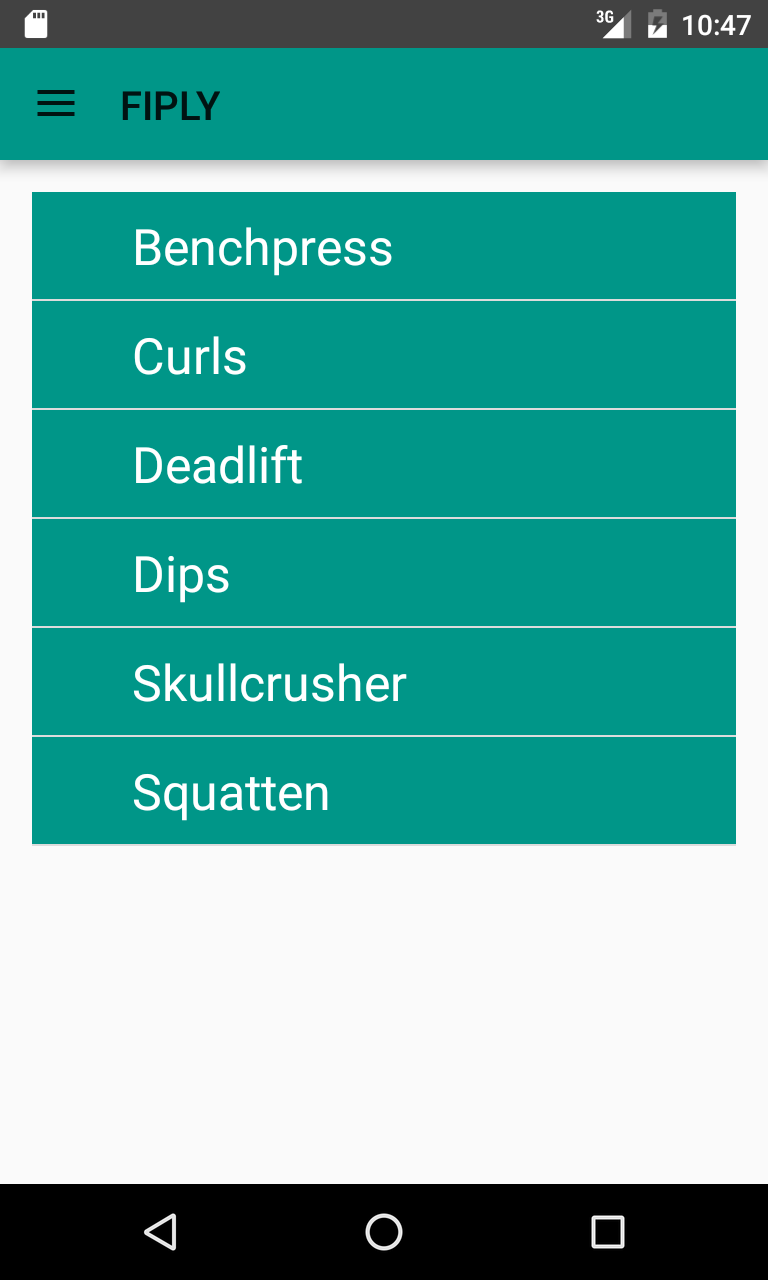
\includegraphics[scale=0.4]{img/Uebungskatalog}

\subsection{DetailView}
Für jede Übung gibt es eine Detailansicht, in welcher man genaures über jene Übung erfahren kann.
\includegraphics[scale=0.4]{img/UebungsKatalog_detail_video }

\begin{itemize}
\item Name der Übung
\item Beschreibung
\item Anleitung
\item Die Muskelgruppe/n welche man mit dieser Übung trainiert.
\item Benötigtes Equipment
\item Ein Video welches die Durchführung beschreibt.
\end{itemize}

Diese Detail-View wird aufgerufen indem man auf die korrespondierende Übung im Übungskatalog tippt.

\subsection{Filter}
\subsubsection{Beschreibung}
Die Liste kann auch nach Name und Muskelgruppe gefiltert werden. 
Der Filter wird über den Floating Action Button aufgerufen.

\subsubsection{Implementierung}
Die Muskelgruppen-Auswahl erfolgt über,das tippen auf eine bestimmte Muskelgruppe,




\end{document}
